%---------------- Description of Industry ----------------%
\section{Description of Industry}

\subsection{Type of Industry}

Campus Glam Hub operates within the personal care and beauty services industry, specifically focusing on the salon and spa sector. This industry encompasses hair care, skincare, makeup, and grooming services. The business falls under the service sector with a retail component for beauty products.

\textbf{Industry Classification:}

According to the Uganda Bureau of Statistics (UBOS) classification system, Campus Glam Hub falls under:
\begin{itemize}[leftmargin=2em]
    \item Sector: Services
    \item Sub-sector: Personal Care Services
    \item Industry: Beauty and Wellness Services
    \item Specific Category: Hair and Beauty Salons
\end{itemize}

\textbf{Industry Characteristics:}

The beauty services industry is characterized by several distinctive features:

Labor-Intensive Nature: The industry relies heavily on skilled labor. Service quality depends primarily on the expertise and skill of beauticians and stylists rather than on capital equipment or technology.

Low Barriers to Entry: Relatively modest capital requirements make it possible for individuals to enter the industry. However, building a successful, sustainable business requires more than just technical skills.

High Competition: The low barriers to entry result in high competition, particularly in urban areas. Differentiation through quality, service, location, or pricing becomes critical for success.

Relationship-Based: Success in the beauty industry often depends on building strong relationships with customers. Repeat business and referrals drive growth more than one-time transactions.

Trend-Sensitive: The industry is highly influenced by fashion trends, celebrity styles, and social media influences. Businesses must stay current with evolving preferences and techniques.

Skill-Dependent: Quality of service delivery depends heavily on the skills and training of service providers. Continuous training and skill development are essential for maintaining competitive advantage.

\textbf{Industry Value Chain:}

The beauty services industry value chain includes:

Product Manufacturers: Companies producing hair care products, cosmetics, and beauty supplies.

Distributors and Wholesalers: Entities that distribute products from manufacturers to retail outlets and service providers.

Beauty Service Providers: Salons, spas, and individual practitioners who deliver services directly to consumers. Campus Glam Hub operates at this level.

Customers: End consumers who purchase services and products.

Supporting Services: Training institutions, equipment suppliers, and industry associations that support the ecosystem.

\subsection{Industry Size and Economic Impact}

\textbf{Global Context:}

The global beauty and personal care market is valued at approximately USD 500 billion annually and growing at 5-6\% per year. The African beauty market, valued at approximately USD 10 billion, is growing faster at 8-10\% annually, driven by rising incomes, urbanization, and increasing beauty consciousness.

\textbf{Ugandan Market Context:}

While comprehensive statistics specific to Uganda's beauty services industry are limited, available data suggests:

The Ugandan beauty and personal care market is estimated at USD 150-200 million annually.

The market has been growing at approximately 8-10\% annually over the past five years.

Urban areas, particularly Kampala and major towns like Mbarara, account for approximately 70\% of the market.

The industry employs an estimated 50,000-100,000 people directly, with many more in supporting roles.

\textbf{Campus Market Specific Context:}

University campuses represent a unique and underserved segment of the beauty services market:

Uganda has over 50 universities and tertiary institutions with a combined student population exceeding 200,000.

Most campuses lack professional beauty service providers, creating significant market opportunity.

Students represent a captive market with consistent demand for beauty services.

Campus-based businesses benefit from lower marketing costs due to concentrated target market and word-of-mouth effectiveness.

\subsection{Future Outlook and Trends of Industry}

The beauty and personal care industry in Uganda is experiencing significant growth, driven by multiple factors:

\textbf{Demographic Trends:}

Youth Population Growth: Uganda has one of the youngest populations globally, with over 75\% under age 30. This demographic is the primary consumer of beauty services.

Urbanization: Increasing urbanization brings more people into areas with access to professional beauty services. Urban population growing at 5-6\% annually.

Rising Middle Class: Economic growth is expanding the middle class, which has greater disposable income for discretionary spending including beauty services.

\textbf{Social and Cultural Trends:}

Increasing Awareness of Personal Grooming: Growing recognition of the importance of personal appearance for professional and social success.

Social Media Influence: Platforms like Instagram, TikTok, and Facebook drive demand for professional styling. Users want to look good in photos and videos they share online.

Changing Beauty Standards: Evolving beauty standards that celebrate diverse looks and natural beauty create demand for various service types.

Professional Expectations: Increasing workplace professionalism expectations drive demand for professional grooming services.

Event Culture: Growing culture of events, celebrations, and social gatherings creates consistent demand for special occasion styling.

\textbf{Economic Trends:}

Growing Disposable Income: Economic growth, even among students through part-time work and family support, increases spending capacity for beauty services.

Service Economy Growth: Shift from agriculture to services in the Ugandan economy creates more opportunities for service-based businesses.

Entrepreneurship Support: Government and private sector initiatives supporting youth entrepreneurship create favorable environment for new businesses.

\textbf{Technology Trends:}

Digital Payment Adoption: Increasing use of mobile money and digital payments makes transactions more convenient.

Social Media Marketing: Low-cost digital marketing through social media platforms enables effective customer reach.

Online Booking Systems: Technology enables convenient appointment scheduling and customer management.

Beauty Tech Products: New beauty technology products and treatments create opportunities for service differentiation.

\textbf{Industry-Specific Trends:}

Natural Hair Movement: Growing acceptance and celebration of natural African hair textures creates demand for specialized natural hair care services.

Male Grooming Acceptance: Increasing acceptance of male grooming services expands the potential market.

Wellness Integration: Beauty services increasingly integrated with wellness and self-care concepts.

Sustainable Beauty: Growing interest in eco-friendly and sustainable beauty products and practices.

Personalization: Increasing demand for personalized services tailored to individual needs rather than one-size-fits-all approaches.

\textbf{Market Growth Projections:}

Based on current trends and economic indicators, the Ugandan beauty services market is projected to:

Grow at 8-10\% annually over the next 5 years.

Reach USD 250-300 million by 2028.

See particularly strong growth in campus-based and convenience-focused services.

Experience increasing professionalization with more trained practitioners and higher service standards.

Benefit from continued urbanization and rising incomes.

\textbf{Campus-Based Services Outlook:}

Campus-based beauty services represent a particularly promising segment:

Underserved Market: Most campuses currently lack professional beauty service providers.

Captive Audience: Students represent a concentrated, accessible market.

Consistent Demand: Academic calendar creates predictable demand patterns.

Growth Potential: As successful models emerge, expansion to multiple campuses becomes viable.

Lower Competition: Fewer competitors compared to urban commercial areas.

The industry is projected to grow at 8-10\% annually in Uganda, with campus-based services showing particularly strong potential due to the captive market and convenience factor.

\subsection{Analysis of Competitors}

Understanding the competitive landscape is essential for positioning Campus Glam Hub effectively. Our competitors fall into several categories, each with distinct characteristics, strengths, and weaknesses.

\textbf{Direct Competitors:}

\textbf{1. Mbarara Town Beauty Salons}

Location and Accessibility: Located 5-10 kilometers from Kihumuro Campus in Mbarara town center. Requires students to arrange transportation, typically costing UGX 2,000-5,000 per trip via boda boda or UGX 1,500-2,000 via taxi.

Service Offerings: Comprehensive beauty services including hair styling, braiding, weaving, makeup, skincare, and nail services. Most offer similar service range to Campus Glam Hub.

Pricing Structure: Services priced 15-25\% higher than Campus Glam Hub's planned pricing. Typical haircut costs UGX 15,000-20,000, braiding UGX 20,000-40,000, makeup UGX 25,000-50,000.

Quality Standards: Generally high quality with trained professionals and professional equipment. Established salons have good reputations for service quality.

Operating Hours: Typically 9:00 AM to 6:00 PM or 7:00 PM, Monday through Saturday. Limited Sunday hours. These hours conflict with class schedules.

Target Market: General population including working professionals, business people, and some students. Not specifically tailored to student needs or budgets.

Strengths:
\begin{itemize}[leftmargin=2em]
    \item Established reputation and customer base
    \item Experienced, trained staff
    \item Professional equipment and facilities
    \item Wide range of services
    \item Strong relationships with product suppliers
\end{itemize}

Weaknesses:
\begin{itemize}[leftmargin=2em]
    \item Distance from campus requires transportation
    \item Higher pricing not optimized for student budgets
    \item Operating hours conflict with class schedules
    \item Not tailored to student preferences and trends
    \item Total cost (service plus transport) significantly higher
\end{itemize}

Market Share: Currently serve approximately 40-50\% of students who use professional beauty services.

\textbf{2. Informal Campus Stylists}

Description: Individual students or community members offering basic beauty services from hostels, homes, or informal settings on or near campus.

Service Offerings: Limited primarily to basic hair braiding, simple hairstyles, and occasional makeup. Rarely offer comprehensive services or specialized treatments.

Pricing Structure: Significantly lower prices, typically UGX 5,000-15,000 for basic services. Price is the primary competitive advantage.

Quality Standards: Highly variable. Some provide acceptable quality, but many lack professional training, proper equipment, or consistent standards. No quality assurance or recourse for unsatisfactory service.

Operating Environment: Informal settings often in hostels or homes. Limited equipment, inconsistent hygiene standards, no professional atmosphere.

Target Market: Price-sensitive students willing to accept lower quality for cost savings.

Strengths:
\begin{itemize}[leftmargin=2em]
    \item Very low prices
    \item Convenient campus location
    \item Flexible hours
    \item Personal relationships with customers
    \item No formal business overhead costs
\end{itemize}

Weaknesses:
\begin{itemize}[leftmargin=2em]
    \item Inconsistent quality
    \item Limited service range
    \item Basic or inadequate equipment
    \item Poor hygiene standards in many cases
    \item No professional training or certification
    \item Unreliable availability
    \item No recourse for poor service
    \item Cannot handle complex services
\end{itemize}

Market Share: Serve approximately 30-40\% of students seeking beauty services, primarily those prioritizing low cost over quality.

\textbf{Indirect Competitors:}

\textbf{3. Mobile Beauty Service Providers}

Description: Individual practitioners or small businesses offering mobile beauty services, traveling to customers' locations.

Service Offerings: Variable depending on provider. Some offer comprehensive services, others specialize in specific areas like makeup or braiding.

Pricing Structure: Moderate to high pricing, typically UGX 10,000-30,000 for basic services, with premium charged for travel and convenience.

Quality Standards: Variable. Some mobile providers are highly skilled professionals, others less so. Quality depends entirely on individual provider.

Operating Model: Customers contact providers via phone or social media to schedule appointments. Provider travels to customer's location with portable equipment.

Strengths:
\begin{itemize}[leftmargin=2em]
    \item Convenience of service at customer's location
    \item Flexible scheduling
    \item Personal service
    \item No need for customer to travel
\end{itemize}

Weaknesses:
\begin{itemize}[leftmargin=2em]
    \item Limited equipment due to portability constraints
    \item Inconsistent availability
    \item Higher prices due to travel time and costs
    \item Unreliable scheduling
    \item Limited service range
    \item Difficulty verifying quality before booking
\end{itemize}

Market Share: Serve approximately 10-15\% of market, primarily for special occasions or customers with specific scheduling constraints.

\textbf{4. DIY and Home Treatments}

Description: Students performing beauty treatments themselves or with help from friends using purchased products.

Service Range: Basic treatments including simple hairstyles, basic makeup, and home skincare routines.

Cost: Only product costs, no service fees. Can be very economical.

Quality: Highly variable depending on individual skill and product quality.

Strengths:
\begin{itemize}[leftmargin=2em]
    \item Lowest cost option
    \item Complete flexibility
    \item Learning opportunity
    \item No appointment needed
\end{itemize}

Weaknesses:
\begin{itemize}[leftmargin=2em]
    \item Limited to simple treatments
    \item Results often inferior to professional services
    \item Time-consuming
    \item Risk of poor results or damage
    \item Cannot achieve complex styles
\end{itemize}

Market Share: Represents approximately 20-30\% of potential market, primarily for basic maintenance between professional services.

\textbf{Competitive Advantages of Campus Glam Hub:}

Against Town Salons:
\begin{itemize}[leftmargin=2em]
    \item Eliminates transportation costs (UGX 4,000-10,000 savings per visit)
    \item Saves 1-2 hours travel time per visit
    \item More convenient scheduling around classes
    \item Lower base pricing (15-20\% less)
    \item Total cost savings of 30-40\%
    \item Extended hours better suited to student schedules
\end{itemize}

Against Informal Stylists:
\begin{itemize}[leftmargin=2em]
    \item Professional quality and consistency
    \item Comprehensive service range
    \item Professional equipment and products
    \item Hygienic, safe environment
    \item Trained, certified staff
    \item Reliable availability and scheduling
    \item Recourse for service issues
    \item Professional atmosphere
\end{itemize}

Against Mobile Services:
\begin{itemize}[leftmargin=2em]
    \item Full range of equipment and services
    \item Consistent availability
    \item Professional facility
    \item More competitive pricing
    \item No scheduling uncertainty
    \item Established location for easy access
\end{itemize}

Against DIY:
\begin{itemize}[leftmargin=2em]
    \item Professional results
    \item Time savings
    \item Access to professional products and equipment
    \item Expert advice and consultation
    \item Complex styles and treatments possible
    \item Reduced risk of poor results or damage
\end{itemize}

\textbf{Competitive Strategy:}

Campus Glam Hub's competitive strategy focuses on occupying the "sweet spot" in the market - offering professional quality at affordable prices with unmatched convenience. We position ourselves as:

More Professional than Informal Stylists: Professional training, equipment, environment, and standards at prices only moderately higher.

More Convenient than Town Salons: On-campus location and student-friendly hours eliminate the primary barriers to accessing professional services.

More Affordable than Town Salons: Lower pricing plus eliminated transportation costs create significant total cost advantage.

More Reliable than Mobile Services: Consistent availability, full equipment range, and professional facility.

More Effective than DIY: Professional results, time savings, and reduced risk justify the cost for important occasions and regular maintenance.

This positioning allows us to capture market share from all competitor categories by offering the optimal combination of quality, convenience, and affordability.

\vspace{1em}

% Competitive Analysis Chart
\begin{center}
\textbf{Competitive Positioning Analysis}
\vspace{0.5em}

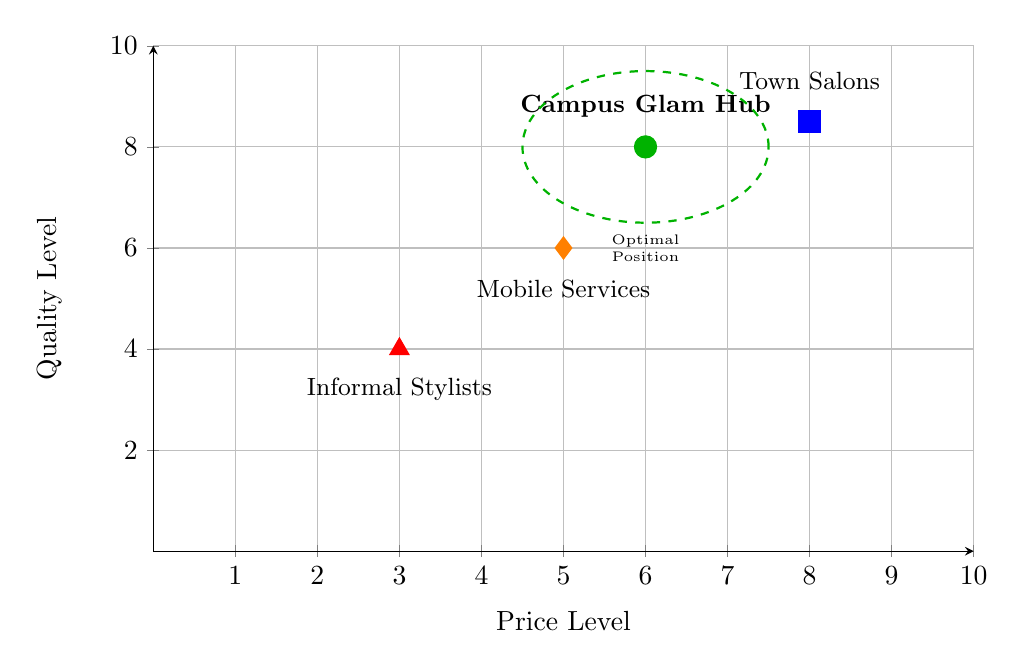
\begin{tikzpicture}
    \begin{axis}[
        xlabel={Price Level},
        ylabel={Quality Level},
        xmin=0, xmax=10,
        ymin=0, ymax=10,
        grid=major,
        width=12cm,
        height=8cm,
        legend pos=north west,
        axis lines=middle,
        xlabel style={at={(axis description cs:0.5,-0.1)},anchor=north},
        ylabel style={at={(axis description cs:-0.1,0.5)},rotate=90,anchor=south}
    ]
    
    % Campus Glam Hub
    \addplot[only marks, mark=*, mark size=4pt, color=green!70!black] 
        coordinates {(6,8)};
    \node at (axis cs:6,8.8) [font=\small\bfseries] {Campus Glam Hub};
    
    % Town Salons
    \addplot[only marks, mark=square*, mark size=4pt, color=blue] 
        coordinates {(8,8.5)};
    \node at (axis cs:8,9.3) [font=\small] {Town Salons};
    
    % Informal Stylists
    \addplot[only marks, mark=triangle*, mark size=4pt, color=red] 
        coordinates {(3,4)};
    \node at (axis cs:3,3.2) [font=\small] {Informal Stylists};
    
    % Mobile Services
    \addplot[only marks, mark=diamond*, mark size=4pt, color=orange] 
        coordinates {(5,6)};
    \node at (axis cs:5,5.2) [font=\small] {Mobile Services};
    
    % Sweet spot circle
    \draw[dashed, thick, color=green!70!black] (axis cs:6,8) circle [radius=1.5];
    \node at (axis cs:6,6) [font=\tiny, text width=2cm, align=center] {Optimal\\Position};
    
    \end{axis}
\end{tikzpicture}

\vspace{0.5em}
Campus Glam Hub occupies the optimal position: high quality at moderate prices, with unmatched convenience.
\end{center}

\vspace{1em}

% Competitive Comparison Table
\begin{center}
\textbf{Detailed Competitor Comparison}
\vspace{0.5em}

\begin{tabular}{|>{\raggedright\arraybackslash}p{2.5cm}|p{2.2cm}|p{2.2cm}|p{2.2cm}|p{2.2cm}|}
\hline
\rowcolor{primarycolor!20}
\textbf{Factor} & \textbf{Campus Glam Hub} & \textbf{Town Salons} & \textbf{Informal Stylists} & \textbf{Mobile Services} \\
\hline
Location & On campus & 5-10 km away & On campus & Variable \\
\hline
Price Range & UGX 10k-50k & UGX 15k-80k & UGX 5k-15k & UGX 10k-30k \\
\hline
Quality & High & High & Low-Medium & Medium \\
\hline
Convenience & Excellent & Poor & Good & Medium \\
\hline
Hygiene & Excellent & Good & Poor & Medium \\
\hline
Equipment & Professional & Professional & Basic & Limited \\
\hline
Service Range & Comprehensive & Comprehensive & Limited & Variable \\
\hline
Reliability & High & High & Low & Medium \\
\hline
\end{tabular}
\end{center}

\subsection{Trends and Market Forecasts}

\textbf{Current Trends:}
\begin{itemize}[leftmargin=2em]
    \item Natural hair care movement gaining popularity among students
    \item Increased demand for event makeup (graduations, parties, photoshoots)
    \item Growing interest in skincare routines and treatments
    \item Male grooming services becoming more accepted
    \item Social media driving demand for trendy hairstyles and makeup looks
\end{itemize}

\textbf{Market Forecast:}
\begin{itemize}[leftmargin=2em]
    \item Expected to capture 30\% of the campus market within the first year
    \item Projected customer base of 150-200 regular clients by month 6
    \item Anticipated 15-20\% growth in customer base annually
    \item Expansion potential to other university campuses in the region
\end{itemize}

